\chapter{Results}\label{ch:results}

\par Here is where I will talk about what I have accomplished.\textbf{\textit{[This totally needs to be actually done]}}
\section{Simulation results, MATLAB}
\par MATLAB was initially used in developing the modified CEs, both with the RLM training method and the NSE training method. The intent of the MATLAB simulation was to verify the potential benefit of both changes to the CE, in an environment where implementing iterational modifications is as frictionless as possible. More realistic analysis, including timing analysis, was conducted in the C++ CE implementation. As such, the SNR profile used in MATLAB-based testing was a simple slow-fading channel. A plot of the SNR profile is shown in Figure \ref{fig:matlabSNRProf}. 

\begin{figure}[ht]
\centering
\includegraphics[scale=1]{figures/matlab_sim_results/snrPRofile_matlabsim.eps}
\caption{SNR profile used in MATLAB simulation.}
\label{fig:matlabSNRProf}
\end{figure}

\par While there are six different fitness score weightings (as shown in Table \ref{table:fitMissions}), the flight tests conducted in \cite{tim_implementation} focused on Emergency, Cooperation and Power Saving. Because of this, these were the missions that the MATLAB simulation focused on as well. Figure \ref{res:matSimFitscore} shows how the fitness score evolved over time during the simulation.

\begin{figure}[ht]
\begin{center}
\begin{subfigure}{\linewidth}
\centering
\includegraphics[scale=0.8]{figures/matlab_sim_results/fitObserved_emer.eps}
\end{subfigure}
\end{center}
\begin{center}
\begin{subfigure}{\linewidth}		
\centering
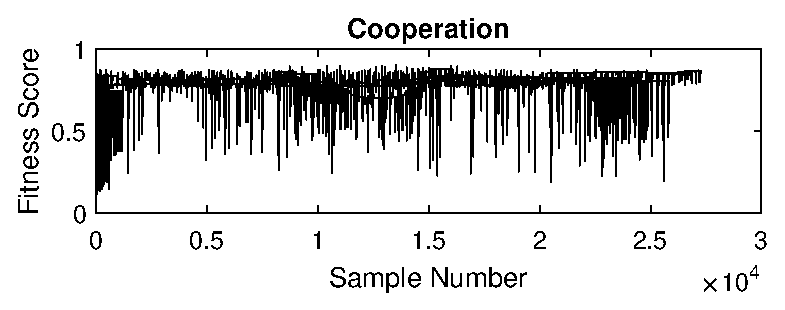
\includegraphics[scale=0.8]{figures/matlab_sim_results/fitObserved_coop.eps}
\end{subfigure}
\end{center}
\begin{center}
\begin{subfigure}{\linewidth}
	\centering
	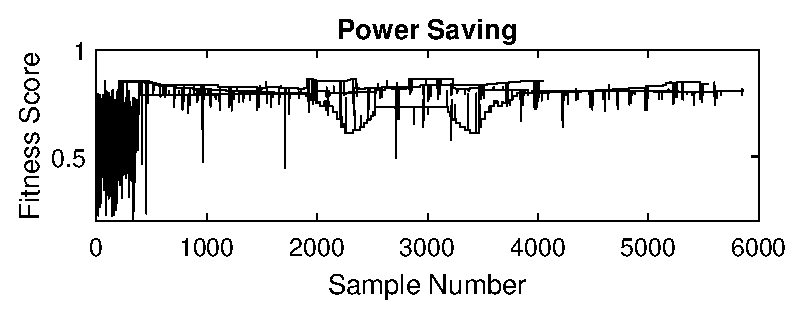
\includegraphics[scale=0.8]{figures/matlab_sim_results/fitObserved_powerSave.eps}
\end{subfigure}
\end{center}
\caption{Fitness score plotted over length of simulation.}\label{res:matSimFitscore}
\end{figure}
\par A few things are evident with the time series plots shown in \ref{res:matSimFitscore}. The first is that the spurs that are periodically showing up are the CE exploring random actions, and are spaced in a manner independent of training type. In addition, it is apparent that some mission types have different ranges of fitness scores that are possible within the action space, as the cooperation simulation has explorations that have a wider range of values than either the emergency simulation or the power saving simulation. Beyond this, it is evident that LM has a more difficult time than the other two training algorithms in adapting to the higher SNR portions of the simulated pass in both the cooperation and powersaving mission cases. Beyond this, it's fairly difficult to draw conclusions from these time series plots.
\begin{figure}[!ht]
\centering
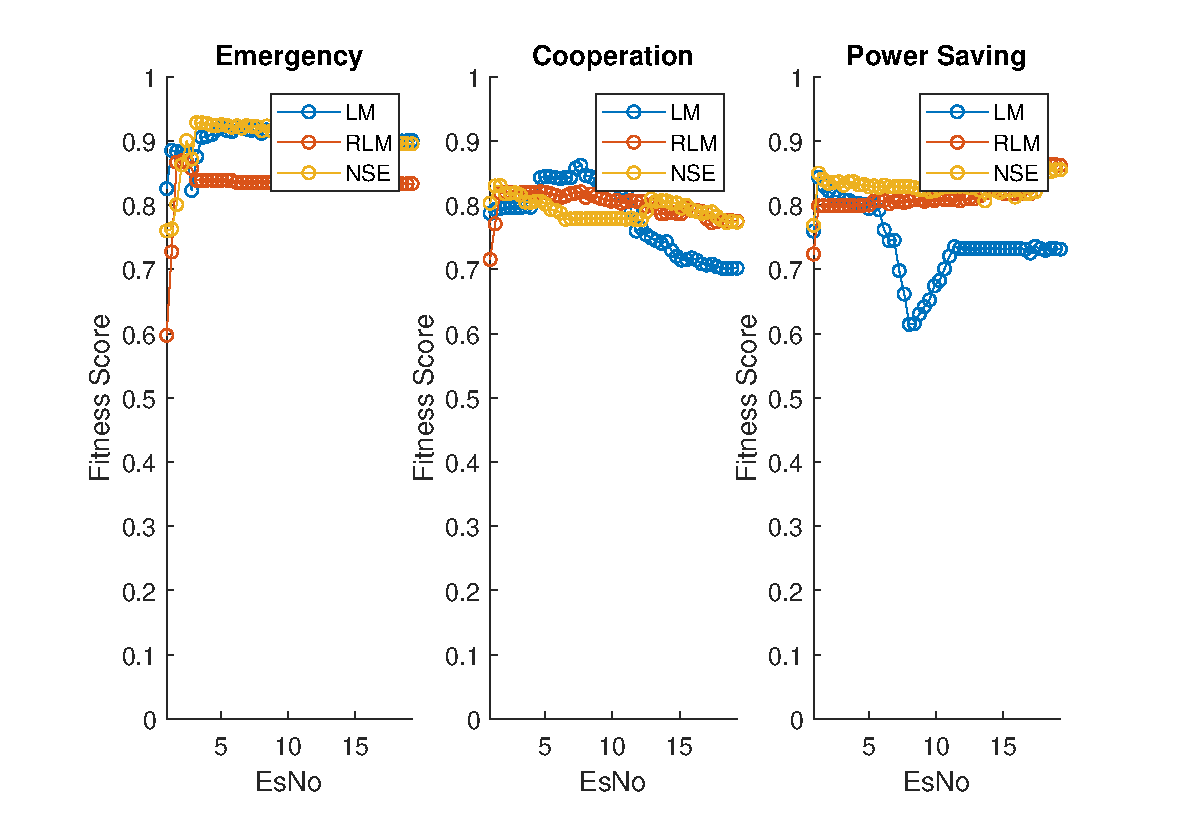
\includegraphics[width=0.8\textwidth]{figures/matlab_sim_results/binnedMeans_sim.eps}
\caption{Value taking the mean fitness value}
\label{res:matSimBinMean}
\end{figure}
\par In order to get a better understanding of the behavior of the different modifications of the CE, fitness scores were split into bins based on the EsNo at the moment that the fitness was observed. Once this was done, the mean was taken within each bin. This plot is shown in Figure \ref{res:matSimBinMean}. For the Emergency mission, LM and NSE proved to have similar average fitness scores, with RLM having lower average fitness scores. The cooperation mission was more ambiguous, with RLM and NSE performing better than LM in the higher EsNo regime, and performing worse than LM in the middle EsNo regime. Finally, the power saving mission shows both LM and RLM working markedly better than LM in the entire regime.
\par With the results shown in this section, there was enough motivation to progress from the MATLAB simulation to simulation, ground testing, and flight testing in C++. 
% \newpage
\section{Simulation results, C++}
\par Simulations using the C++ implementation of the CE served two main purposes. The first purpose of C++ simulations was to verify the correct operation of the code. The second purpose is to provide a completely identical EsNo profile with which to compare the different training algorithms. As much as the NASA flight staff intended to use useful and consistent metrics when evaluating the quality of the communications channel during the window of opportunity when the ISS can be communicated with, the variation of conditions within each quality category resulted in the different tests conducted between 2017 and 2018 having pass qualities that were \textit{fairly\textbf{[this word is probably too vague]}} different from each other, making them harder to directly compare. Running a simulation allows for more direct comparison, albeit without the possibility of shifting the action space in a way that breaks the communication link.
\par The SNR profiles used in the C++ simulation come from attenuation profiles that were measured by NASA employees at GRC. These profiles are used with variable attenuators to simulate channel conditions. By subtracting these values from the maximum EsNo that the CE is expected to see, the attenuation. These values were fed to the CE. One example pass is shown in Figure \ref{result:cSimSNRProfile}, while the rest can be found in Appendix \ref{app:cSNRProfiles_all}. 

\begin{figure}[ht]
\centering
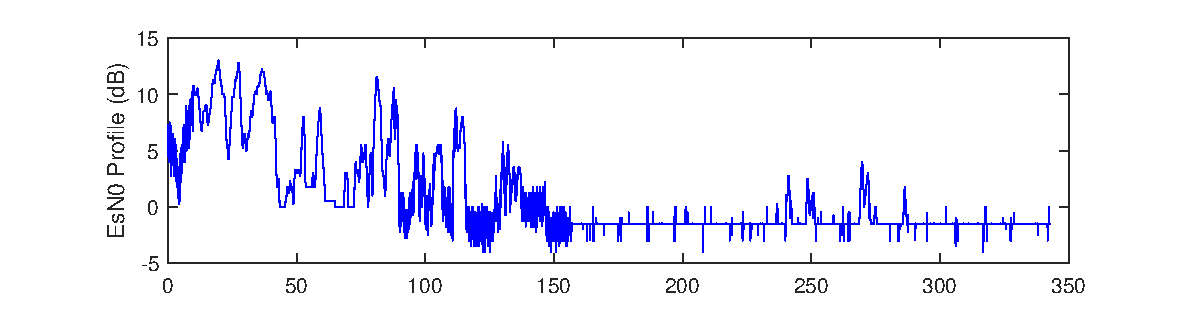
\includegraphics[scale=1]{figures/c_sim_results/sim22_SNRProfile.eps}
\caption{One of the SNR profiles used in C++ simulation.}
\label{fig:cSimSNRProfile}
\end{figure}
\par The EsNo profile for the C++ simulation are significantly more complex than the EsNo profile used in the MATLAB simulation. This is because of the fact that the C++ simulation uses measurements taken from the channel instead of modelling the channel with a simple slow fade property. One of the key differences between LM and the new algorithms being studied is that both RLM and NSE have benefits of pretraining. RLM can explicitly learn a better representation of the environment, while NSE can build up a cache of pretrained networks. LM, on the other hand, will replace the information learned in pretraining, and so did not utilize pretraining. 
\par Running the C++ CE implementation generates a logging file, containing the salient information from each iteration of the algorithm, including the time it takes to choose an action, the fitness score observed, and the other evaluation parameters that combine to become the fitness score. Figure \ref{fig:c22LMCoop} is a summary of the CE running LM operating the cooperation mission on the SNR profile shown earlier. The same plots for RLM and NSE are shown in Figures \ref{fig:c22RLMCoop} and \ref{fig:c22NSECoop} respectively. The key difference that's noticable from this series of plots is that RLM takes a significantly longer amount of time to train, as expected. The plots also provide some intuition about what the action space is actually representing. Even with this, this set of visualizations is hard to utilize for comparison between training algorithms.
\begin{figure}[ht]
\centering
\begin{subfigure}{\linewidth}
	\centering
	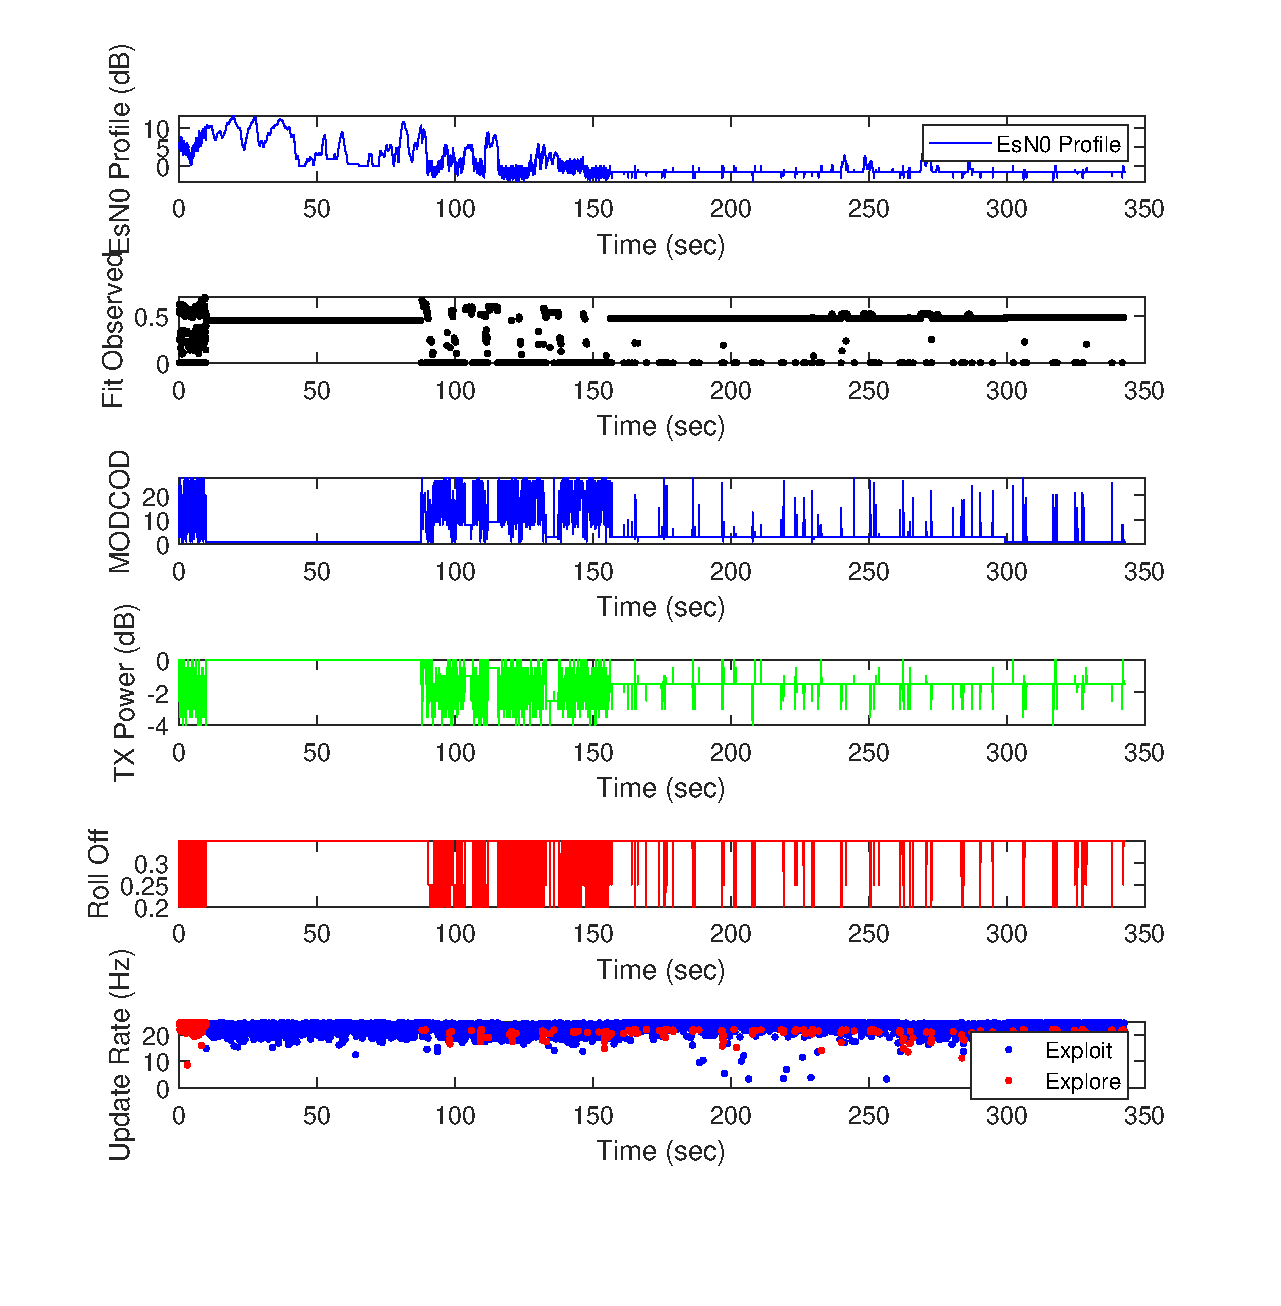
\includegraphics[scale=0.5]{figures/c_sim_results/sim22_LM_overview_coop.eps}
	\caption{Overview of LM operating cooperation mission.}
	\label{fig:cSimLMOverview}
\end{subfigure}\\
\begin{subfigure}{\linewidth}
	\centering
	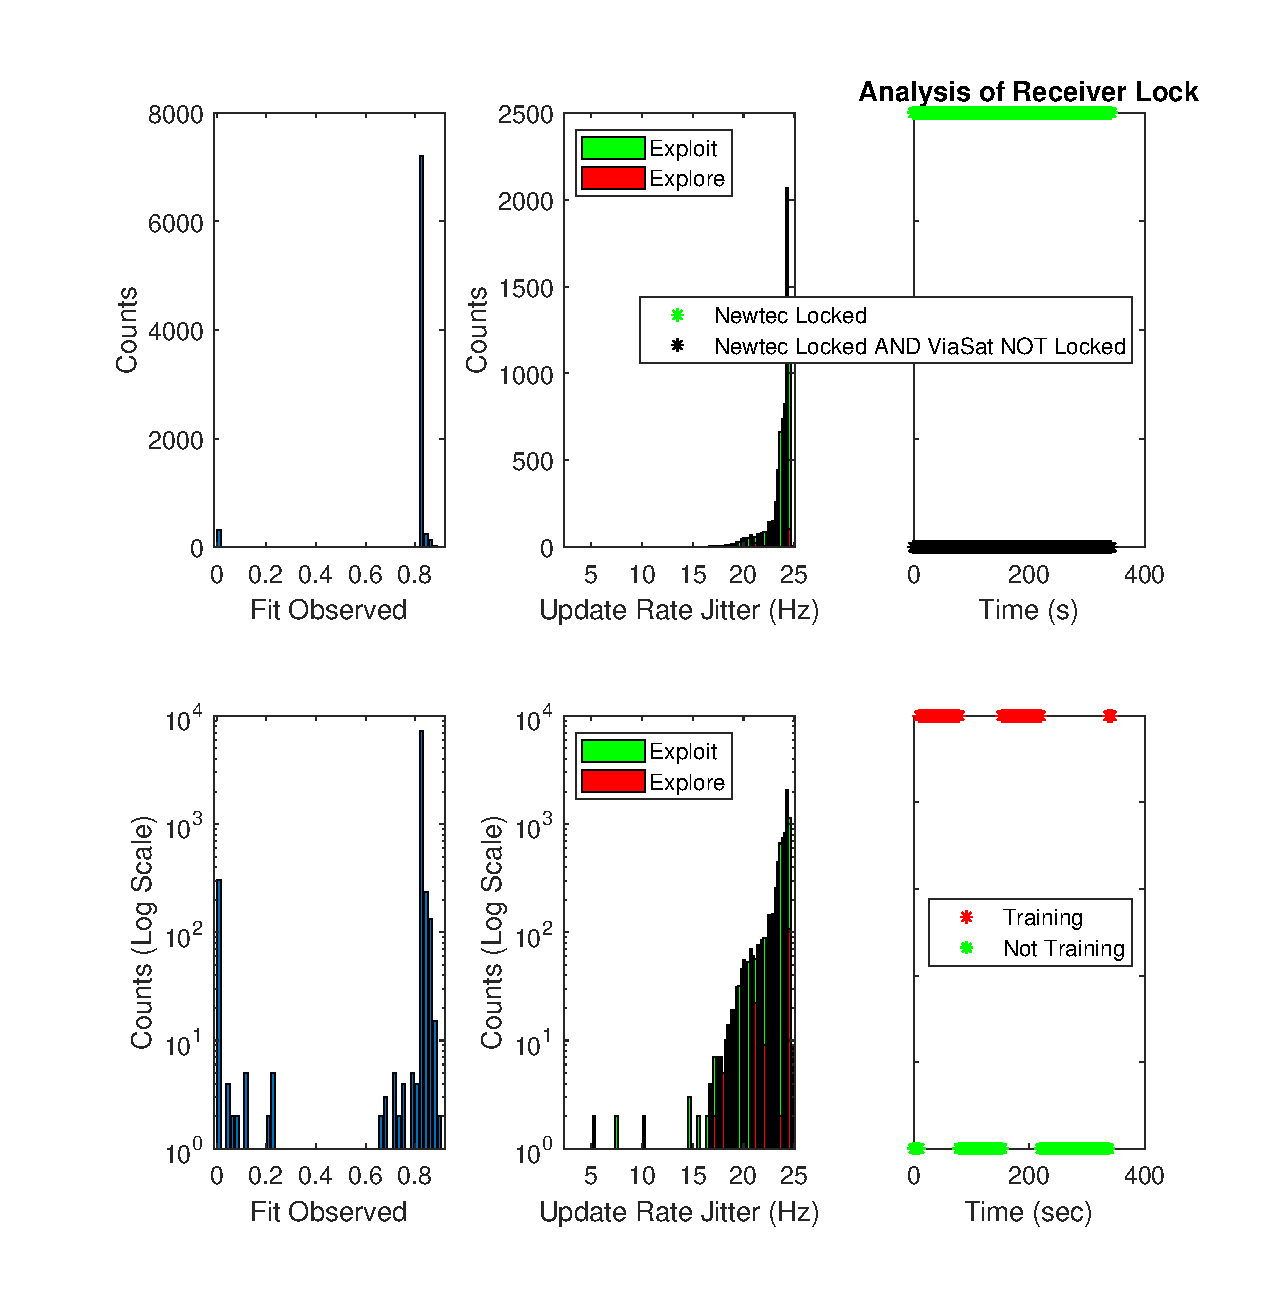
\includegraphics[scale=0.5]{figures/c_sim_results/sim22_LM_hists_coop.eps}
	\caption{Histogram of LM operating cooperation mission. \textit{\textbf{[make this text more interesting]}}}
	\label{fig:cSimLMHists}
\end{subfigure}
\caption{Summary of CE-LM operation with cooperation mission on the pass in Figure \ref{fig:cSimSNRProfile}.}
\label{fig:c22LMCoop}
\end{figure}
\begin{figure}[ht]
\centering
\begin{subfigure}{\linewidth}
	\centering
	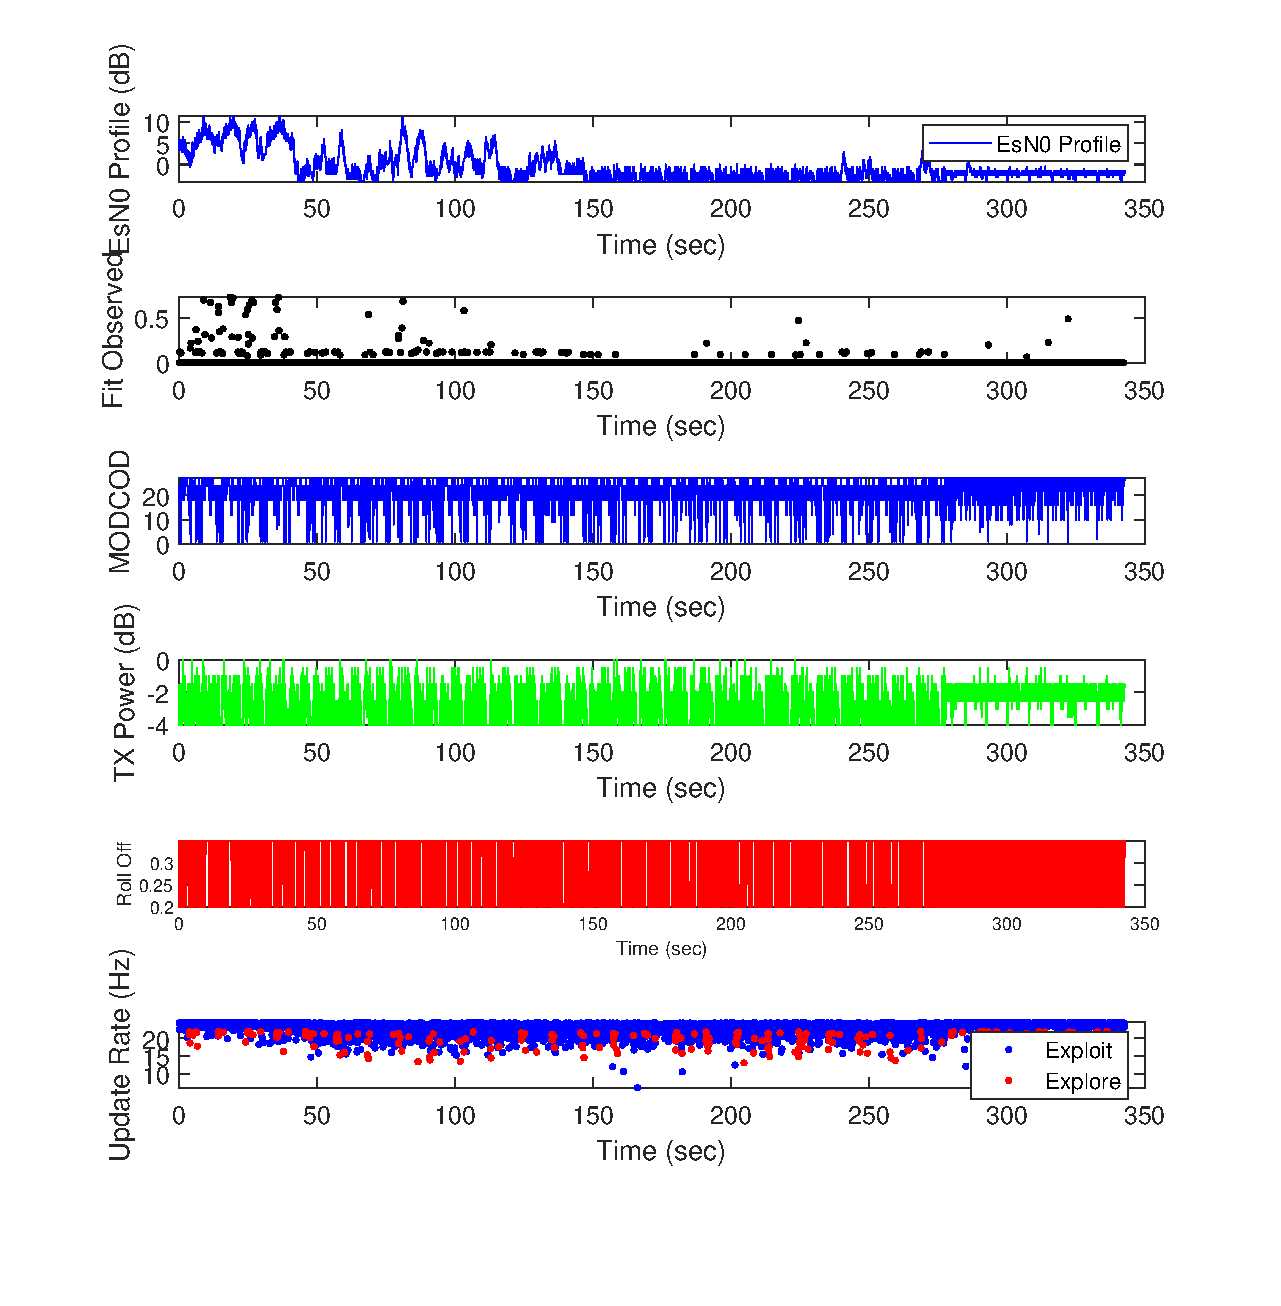
\includegraphics[scale=0.5]{figures/c_sim_results/sim22_RLM_overview_coop.eps}
	\caption{Overview of RLM operating cooperation mission.}
	\label{fig:cSimLMOverview}
\end{subfigure}\\
\begin{subfigure}{\linewidth}
	\centering
	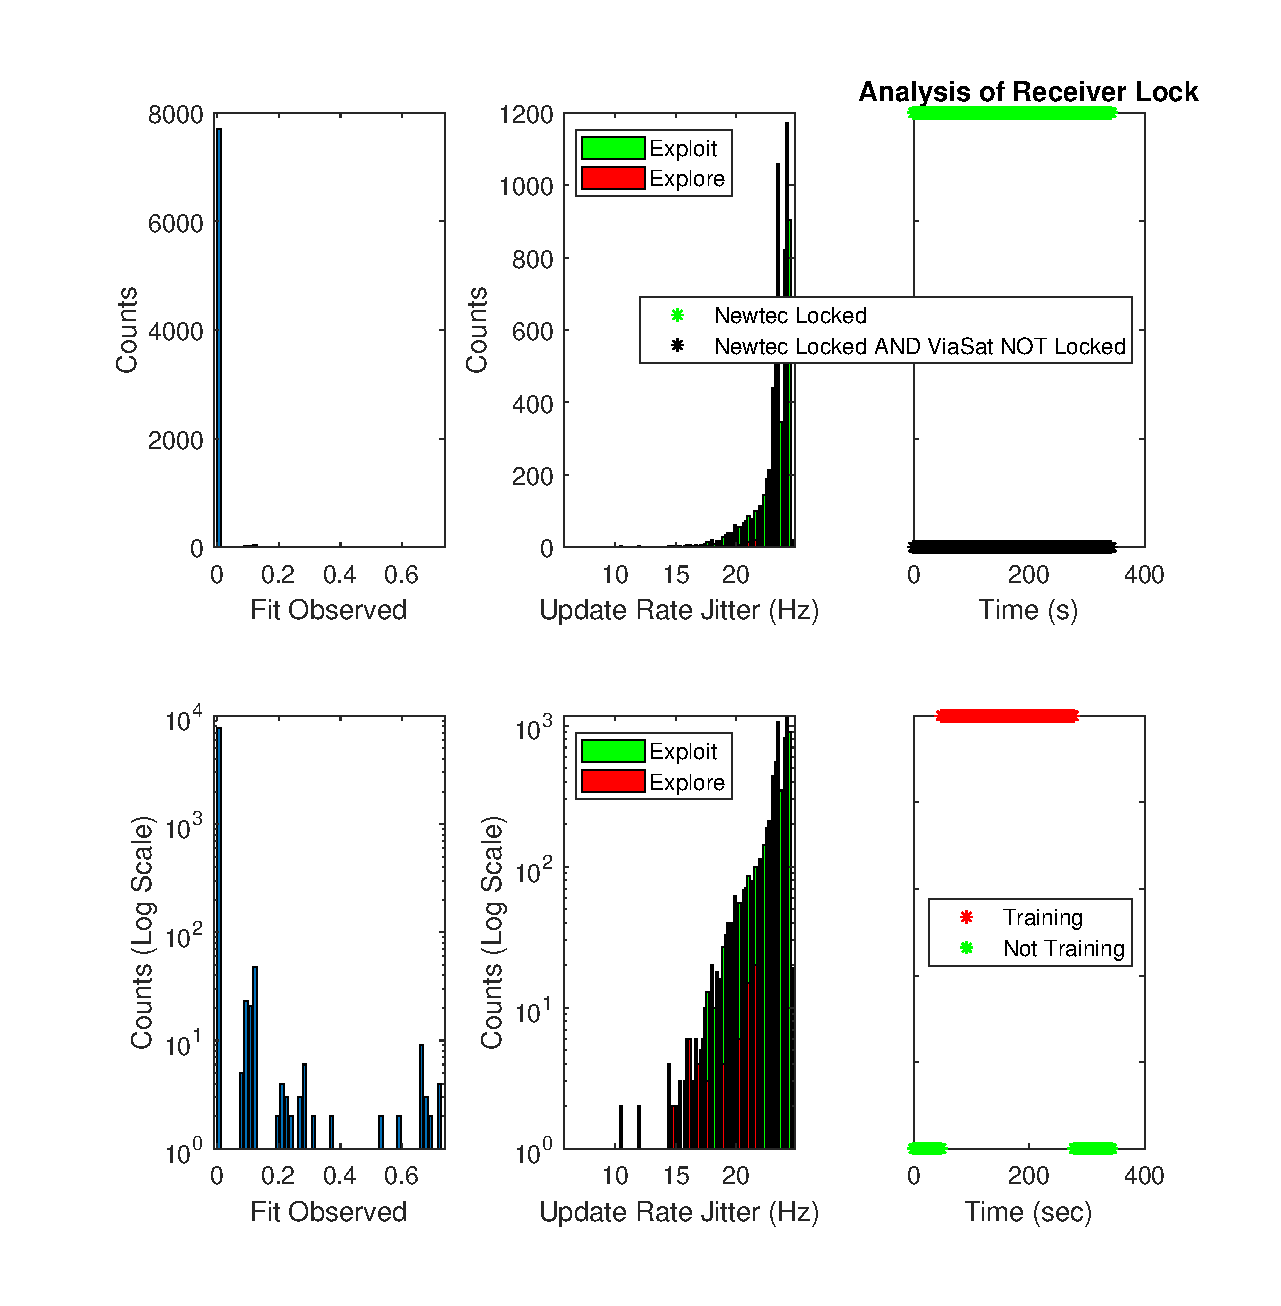
\includegraphics[scale=0.5]{figures/c_sim_results/sim22_RLM_hists_coop.eps}
	\caption{Histogram of RLM operating cooperation mission. \textit{\textbf{[make this text more interesting]}}}
	\label{fig:cSimLMHists}
\end{subfigure}
\caption{Summary of CE-RLM operation with cooperation mission on the pass in Figure \ref{fig:cSimSNRProfile}.}
\label{fig:c22RLMCoop}
\end{figure}
\begin{figure}[ht]
\centering
\begin{subfigure}{\linewidth}
	\centering
	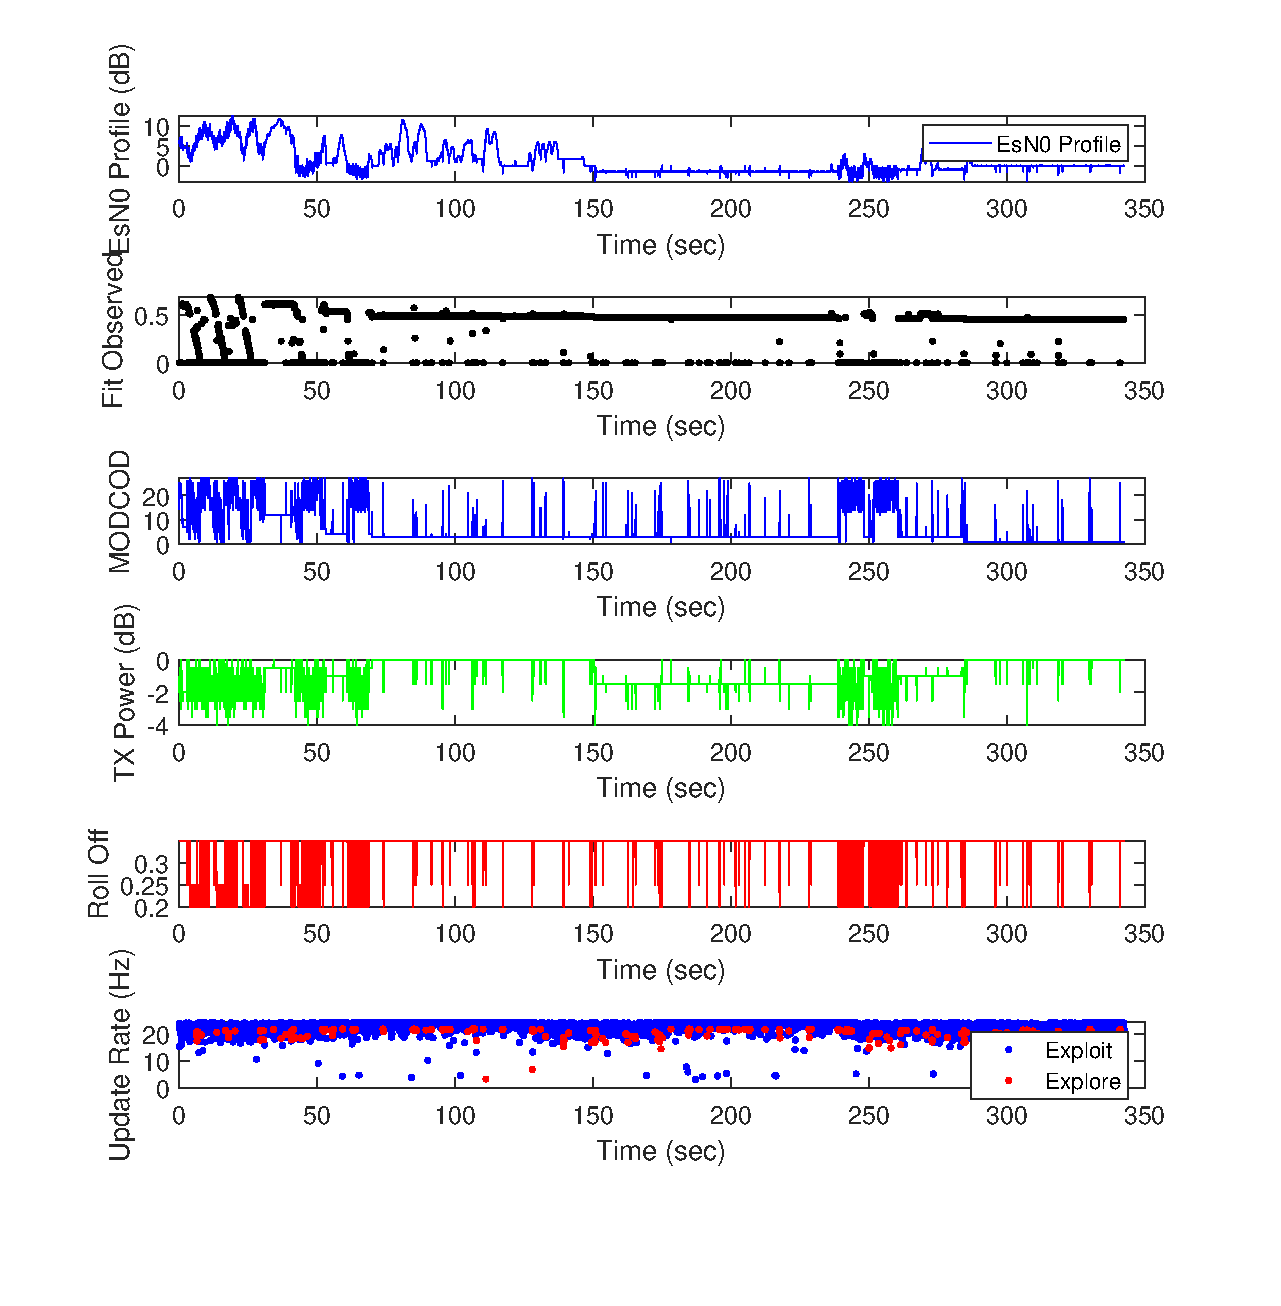
\includegraphics[scale=0.5]{figures/c_sim_results/sim22_NSE_overview_coop.eps}
	\caption{Overview of NSE operating cooperation mission.}
	\label{fig:cSimNSEOverview}
\end{subfigure}\\
\begin{subfigure}{\linewidth}
	\centering
	\includegraphics[scale=0.5]{figures/c_sim_results/sim22_NSE_hists_coop.eps}
	\caption{Histogram of NSE operating cooperation mission. \textit{\textbf{[make this text more interesting]}}}
	\label{fig:cSimNSEHists}
\end{subfigure}
\caption{Summary of CE-NSE operation with cooperation mission on the pass in Figure \ref{fig:cSimSNRProfile}.}
\label{fig:c22NSECoop}
\end{figure}


\clearpage

\par Like the MATLAB simulation, the fitness scores were binned by EsNo, and the mean and median were taken within each bin. Unlike the MATLAB simulation, however, the postprocessing of the CE log files includes the calculation of the optimal action to be taken during each iteration, given the last observed state. This was left out of the MATLAB simulation as all the training methods would use the same pass, and so could be compared easier than results from the flight test. Because this was already built into the postprocessing script, the C++ simulations utilize this optimal action and fitness score in evaluation. Using the optimal fitness score acheivable, the fitness values observed are normalized by subtracting them from the optimal fitness value that was observable at any given action. This will be referred to as the fitness distance. This fitness distance replaces the raw fitness scores in the process of calculating binned means and medians.
\begin{figure}[ht]

\begin{subfigure}{0.50\linewidth}
\centering
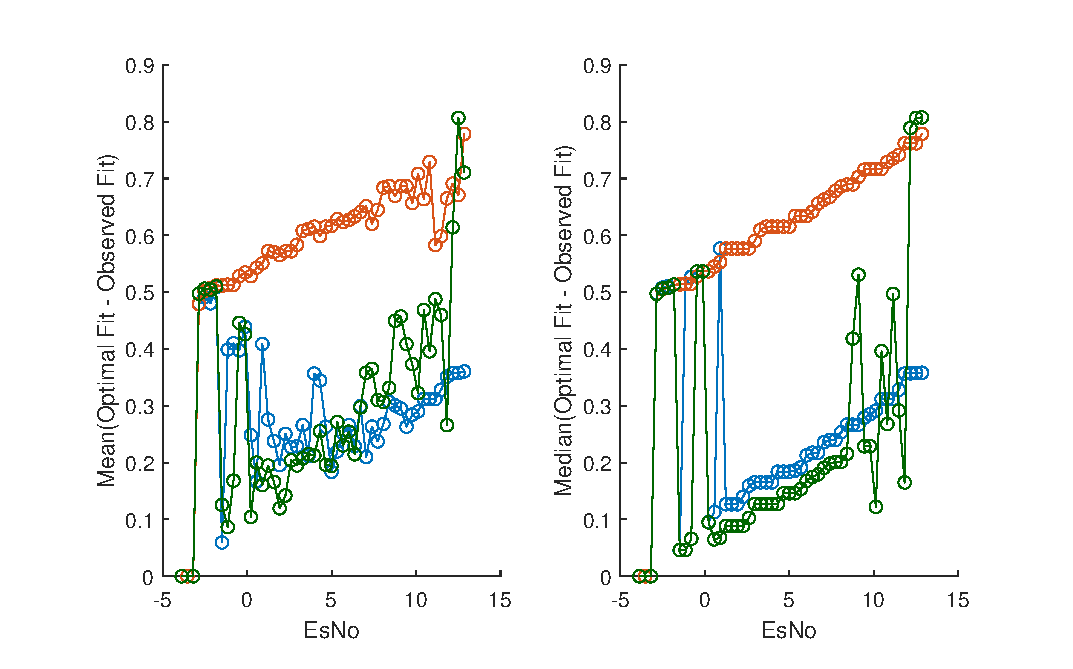
\includegraphics[scale=0.6]{figures/c_sim_results/sim22_binnedMeanMedian.eps}
\caption{Mean and median \textit{\textbf{[make this actually a good caption lol]}}}
\label{fig:cSimBinMeanMed}
\end{subfigure}%
\begin{subfigure}{0.50\linewidth}
\centering
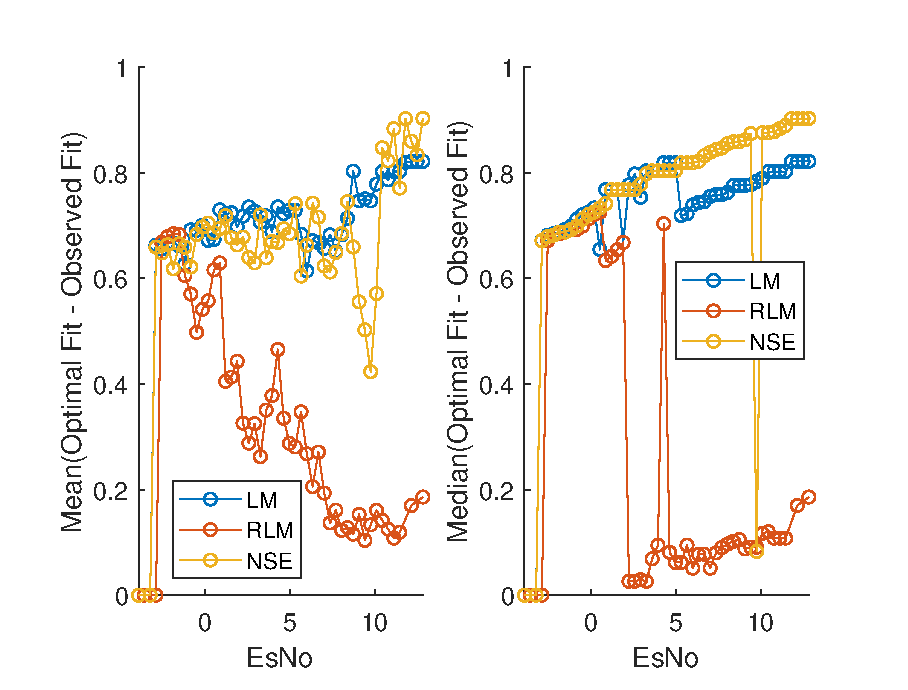
\includegraphics[scale=0.6]{figures/c_sim_results/sim22_binnedMeanMedian_powersave.eps}
\caption{Mean and median \textit{\textbf{[make this actually a good caption lol]}}}
\label{fig:cSimBinMeanMedPwr}
\end{subfigure}
\caption{[fillercaption]}
\label{fig:cSimBinMeanMed}
\end{figure}

\par The binned mean and median plots are shown in Figure \ref{fig:cSimBinMeanMedCoop}. The first notable observation is that CE-RLM performed significantly worse than either CE-LM or CE-NSE. \textit{I have been attributing this behavior to the RLM algorithm requiring more training to properly converge vs the other algorithms, which combined with the extended time it takes to train is making it not converge at all. \textbf{[make this actually make sense]}}. This behavior seems to be situational to the individual pass and performance combination. For instance, running the power saving mission on the same EsNo profile results in CE-RLM outperforming CE-NSE and CE-LM. This is shown in Figure \ref{fig:cSimBinMeanMedPwr}. \textit{\textbf[come up with some explanation for this discrepancy]}.  

\par The binned mean and median representations allow for a simple evaluation of performance between the training methods, but is potentially an oversimplification. A different representation of the data is shown in Figure \ref{fig:cSimBin2dHist}. In this figure, a 2 dimensional histogram is taken. One dimension is the EsNo bins, much in the same way as the binned means. The other dimension is the fitness distance observed. The counts are then put on a log scale. This style of plot makes it easier to understand what the CE is actually doing. Each visible line represents an action or cluster of actions selected by the CE. At lower EsNo values, these actions approach the best action that can be taken. When the CE has identified an action that functions well, it tends to not explore far enough to locate one that may work better. This is the reason behind the same action continuing to be chosen for higher EsNo values. The consistent bar of high fitness distance actions in the plots represent the failure case of the CE, when the action chosen reports zero fitness. This is consistent through all of the 2d plots. More of these plots are shown in appendix \ref{app:2dHistSim}.

\begin{figure}
\centering
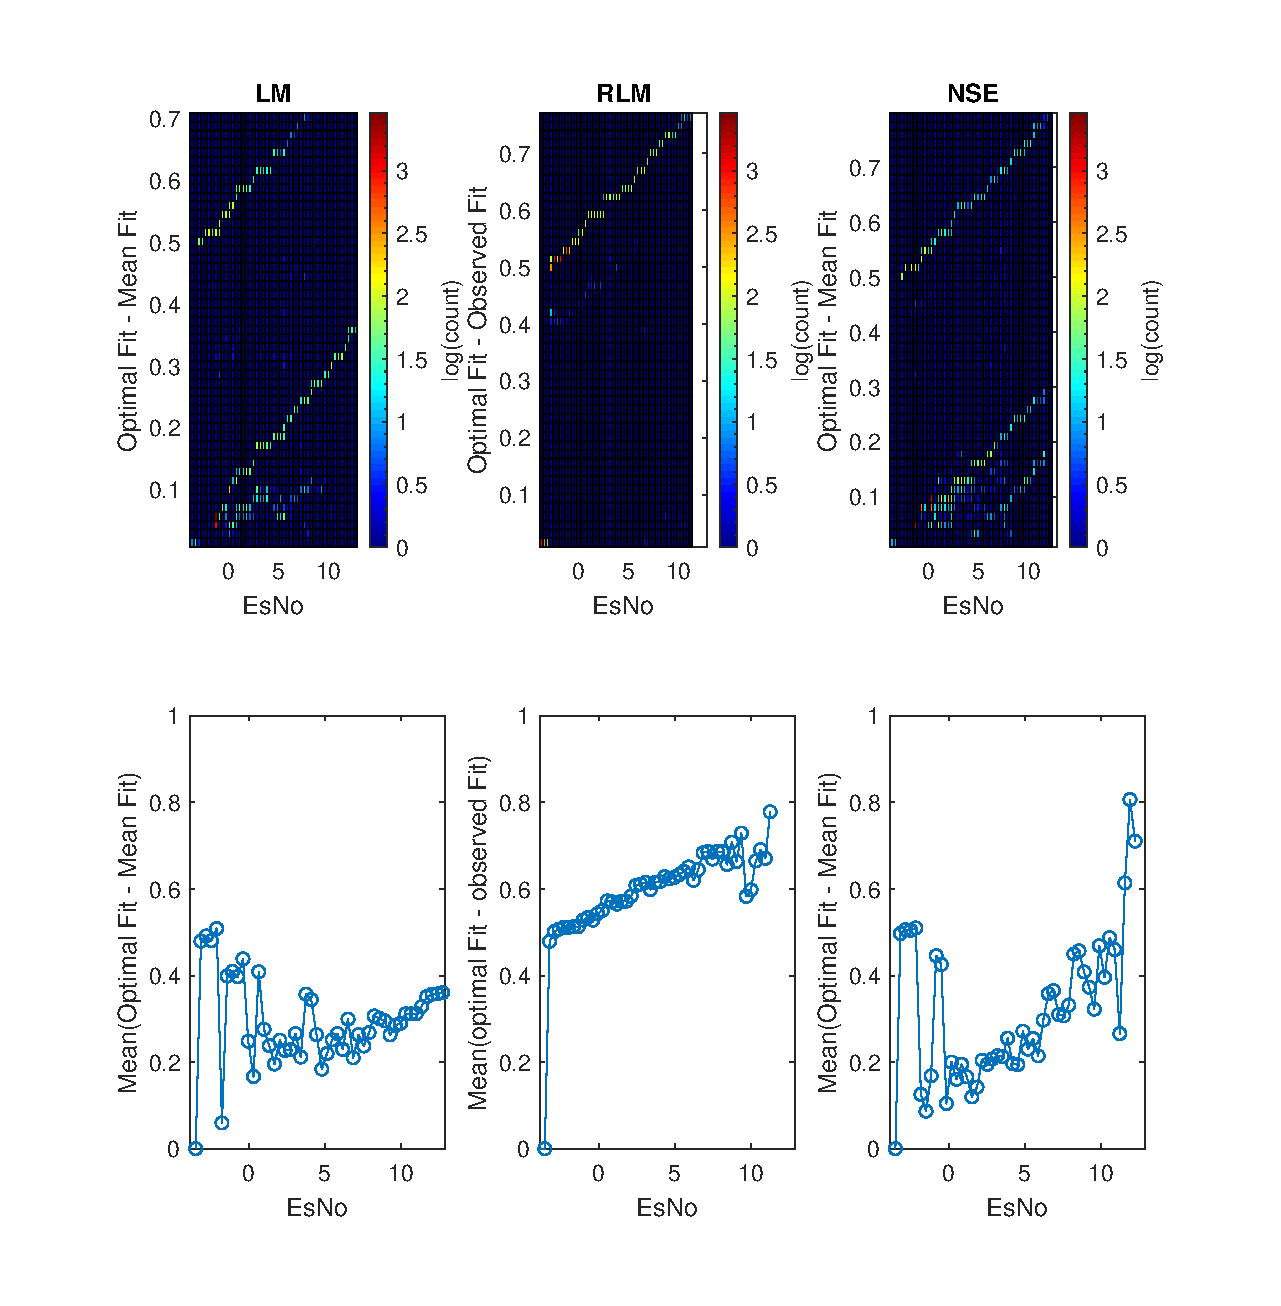
\includegraphics[scale=0.8]{figures/c_sim_results/sim22_2dhist.eps}
\caption{2dHist \textit{\textbf{[make this actually a good caption lol]}}}
\label{fig:cSimBin2dHist}
\end{figure}

\par In order to approach a single-number evaluation of the performance of the different training methods, the binned mean fitness distances for each method is compared. For each pass used, the difference is taken between the fitness distances of  LM and NSE, LM and RLM, and RLM and NSE. This difference turns out positive if the first method in the difference has a higher fitness distance than the second method, implying the second method performed better. Likewise, this number is negative if the second method has a higher fitness distance than the first method. The difference in means is then summed up. This is done for each of the simulations, and is shown in Figure \ref{fig:unweight_sumFit}.
\begin{figure}[ht]

\begin{subfigure}{0.55\linewidth}
	\centering
	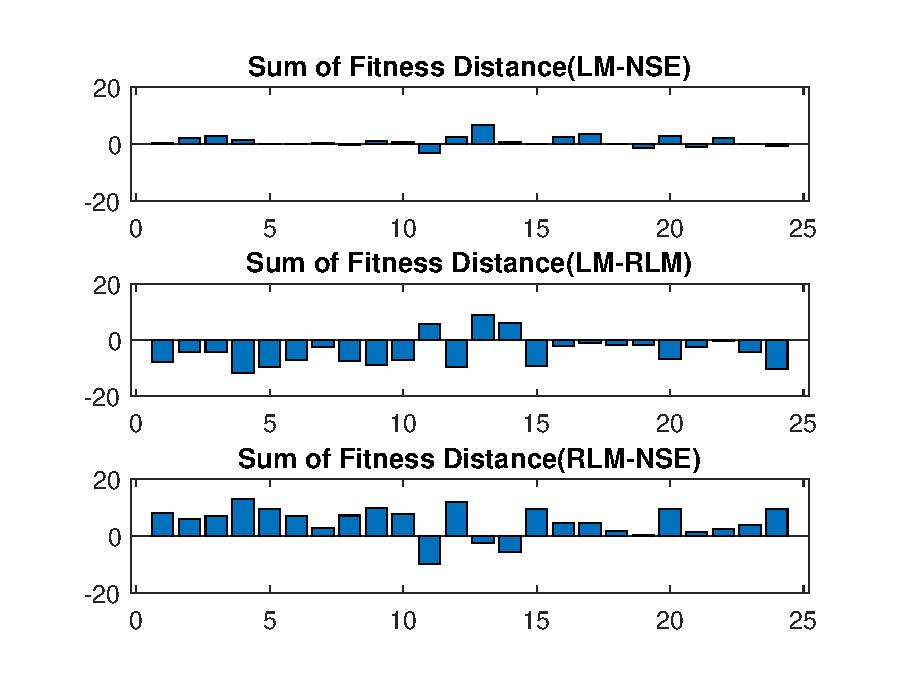
\includegraphics[scale=0.6]{figures/c_sim_results/emer_unweighted_sumFitness.eps}
	\caption{[emergency, fillercaption]}
	\label{fig:cSimUnweightEmer}
\end{subfigure}%
\begin{subfigure}{0.55\linewidth}
	\centering
	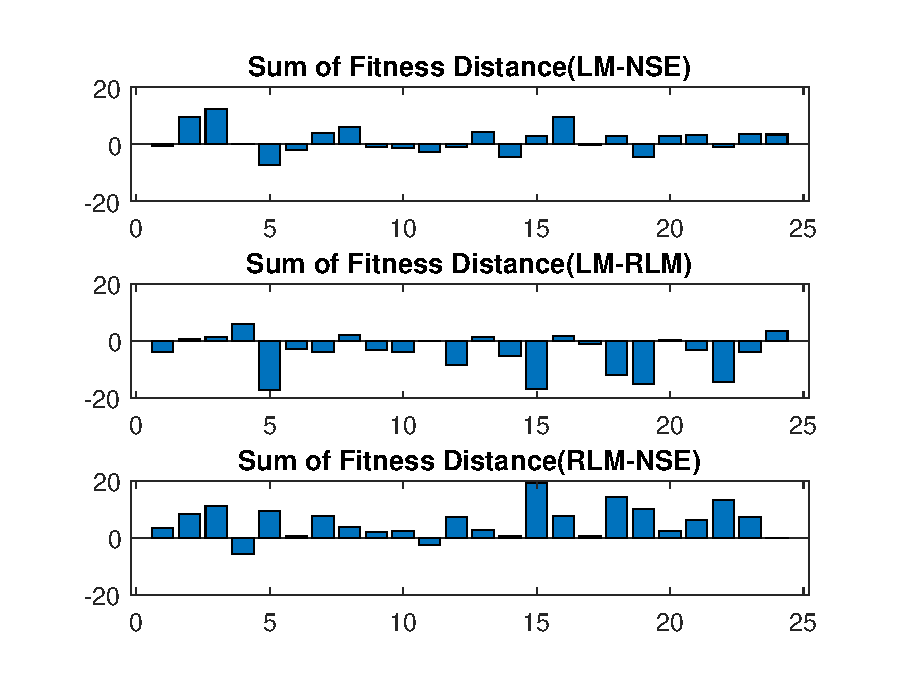
\includegraphics[scale=0.6]{figures/c_sim_results/coop_unweighted_sumFitness.eps}
	\caption{[coop, fillercaption]}
	\label{fig:cSimUnweightCoop}
\end{subfigure}\\
\begin{center}
\begin{subfigure}{0.55\linewidth}
	\centering
	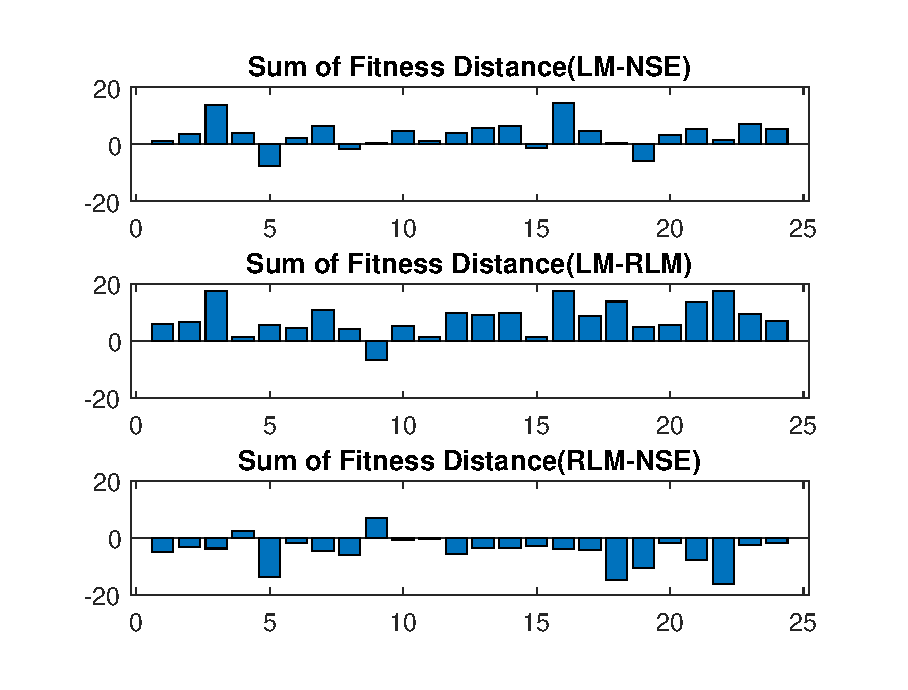
\includegraphics[scale=0.6]{figures/c_sim_results/power_unweighted_sumFitness.eps}
	\caption{[power, fillercaption]}
	\label{fig:cSimUnweightPower}
\end{subfigure}
\end{center}
\caption{[fillercaption.]}
\label{fig:unweight_sumFit}
\end{figure}

\par For the Emergency and Cooperation missions, It is fairly clear that CE-NSE outperforms CE-RLM, with the majority of the fitness distance sums being positive. Looking at Figure \ref{fig:cSimLMOverview}, this appears likely due to the fact that the exploit networks having not properly converged to an action given the EsNo behavior. However, as mentioned before this isn't always the case, as CE-RLM outperforms both CE-LM and CE-NSE for most SNR profiles during the Power Saving mission. For all missions, CE-NSE appears to have modest improvements on the performance of CE-RLM overall. The moderate but not overwhelming improvements can be attributed to the fact that the base learning algorithm is the same, and all the improvements come from clever usage of ensembles.

\begin{figure}[ht]

\begin{subfigure}{0.55\linewidth}
	\centering
	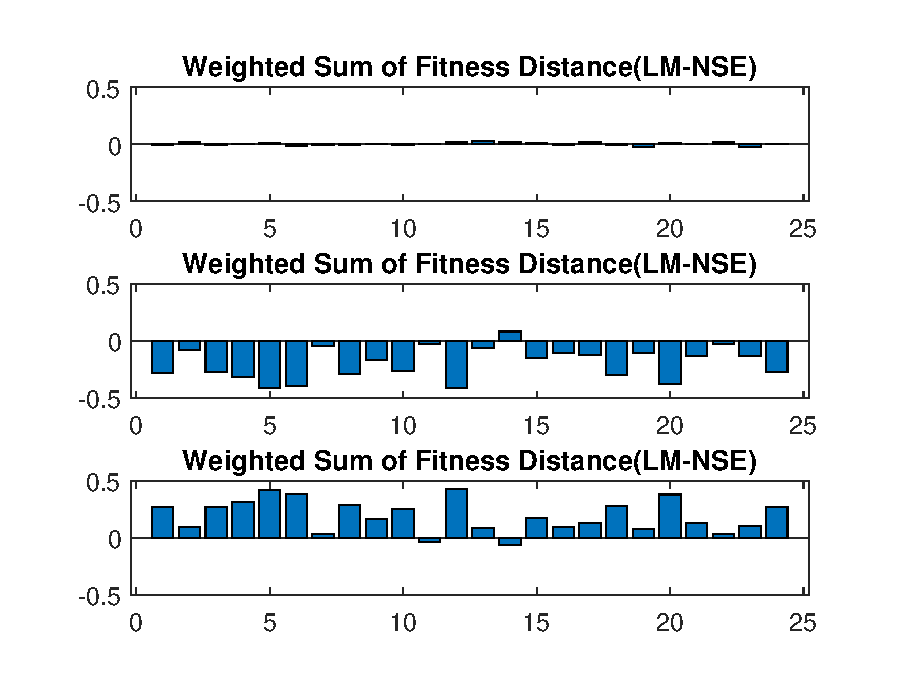
\includegraphics[scale=0.6]{figures/c_sim_results/emer_weighted_sumFitness.eps}
	\caption{[emergency, fillercaption]}
	\label{fig:cSimWeightEmer}
\end{subfigure}%
\begin{subfigure}{0.55\linewidth}
	\centering
	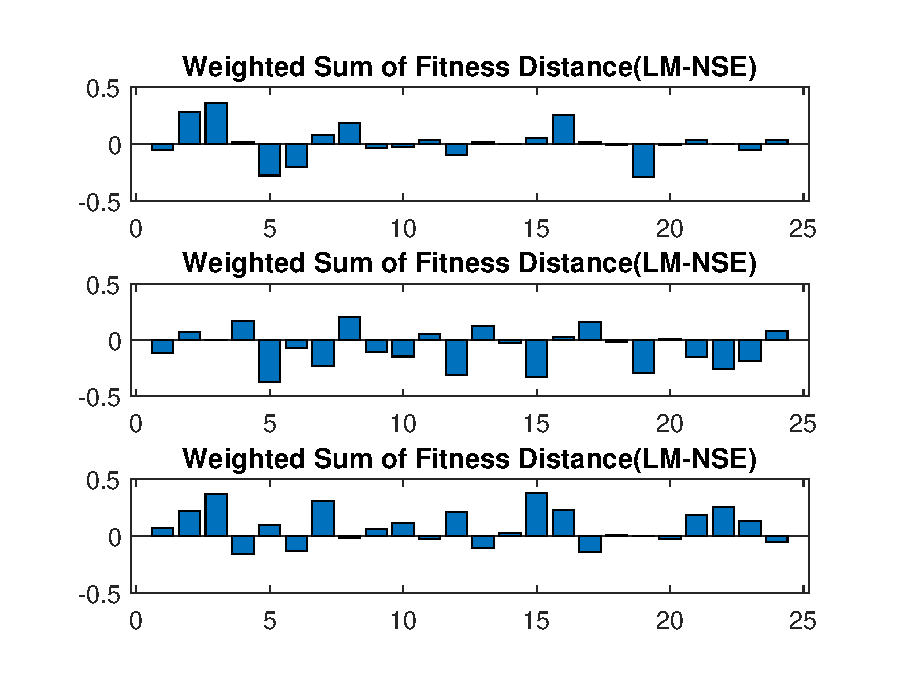
\includegraphics[scale=0.6]{figures/c_sim_results/coop_weighted_sumFitness.eps}
	\caption{[coop, fillercaption]}
	\label{fig:cSimWeightCoop}
\end{subfigure}\\
\begin{center}
\begin{subfigure}{0.55\linewidth}
	\centering
	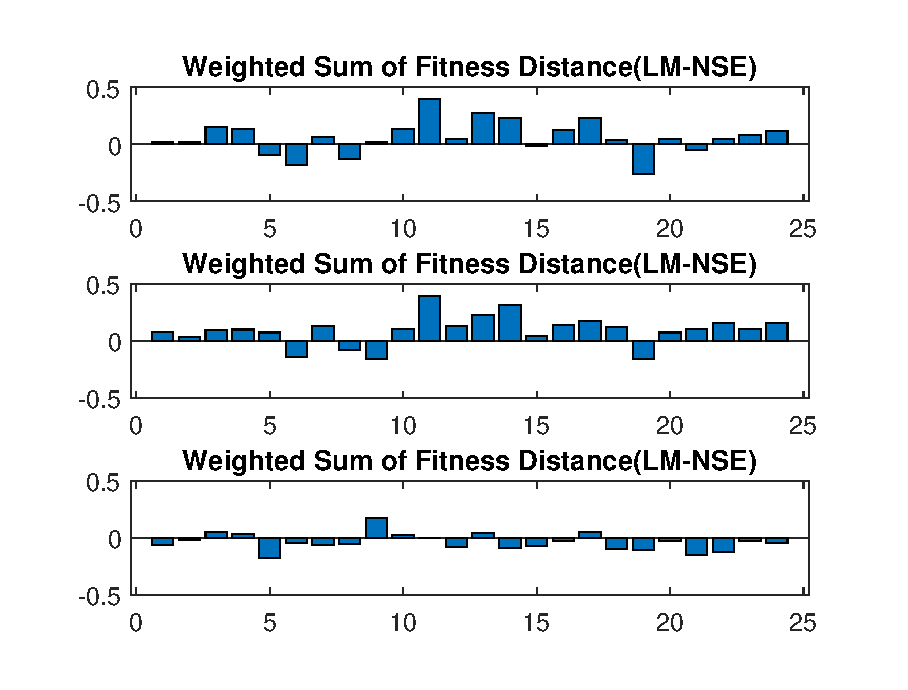
\includegraphics[scale=0.6]{figures/c_sim_results/power_weighted_sumFitness.eps}
	\caption{[power, fillercaption]}
	\label{fig:cSimWeightPower}
\end{subfigure}
\end{center}
\caption{[fillercaption.]}
\label{fig:weight_sumFit}
\end{figure}

\par One potential flaw of the plots in Figure \ref{fig:unweight_sumFit} is that a bin that has a small number samples in it would have the same impact on the plot as a bin that has a large samples in it. In order to mitigate this, the same plots were recalculated, except the mean and median values of the bins were multiplied by the number of samples in the bin divided by the total number of samples. This way, a good performance in a common EsNo regime won't be overshadowed by a poor performance in an uncommon EsNo regime. These modified plots are shown in Figure \ref{fig:weight_sumFit}. This normalization changed some of the results for individual SNR profiles, but the general patterns observed remain the same.
\section{Flight Test results}
\par Flight tests were conducted in two different time periods: the testing of CE-LM were conducted between May 2, 2017 and May 12, 2017, as described in \cite{tim_implementation_paper}. The testing of the new training methods occurred between August 16, 2018 and August 24, 2018. Tables containing more details about the conditions in which the training methods were tested are included in Appendix \ref{app:tables_with_pass_details}. 
\par The quality of passes were split into qualitative categories: Excellent/Great, Good, and OK/Poor. Excellent and Great (as well as OK and Poor) are separate categories, but have been combined during processing as a result of the limited amount of time for testing. As stated previously, these categories were determined by the NASA flight staff, and were related to the amount of time where the EsNo was above certain thresholds. 
\begin{figure}[ht]
\centering
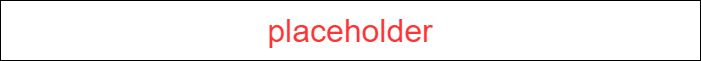
\includegraphics[scale=0.5]{figures/Placeholder.png}
\caption{Placeholder. \textbf{\textit{Will have the overview plot from before, as well as timing histogram plot. A whole lot of formatting is needed and I'm running out of steam today.}}}
\end{figure}
\par \textbf{\textit[paragraph walking through the different passes]}
\begin{figure}[ht]
\centering
\includegraphics[width=\textwidth]{figures/flight_results/Coop_great_overview.eps}
\caption{Placeholder}
\end{figure}
\begin{figure}[ht]
\centering
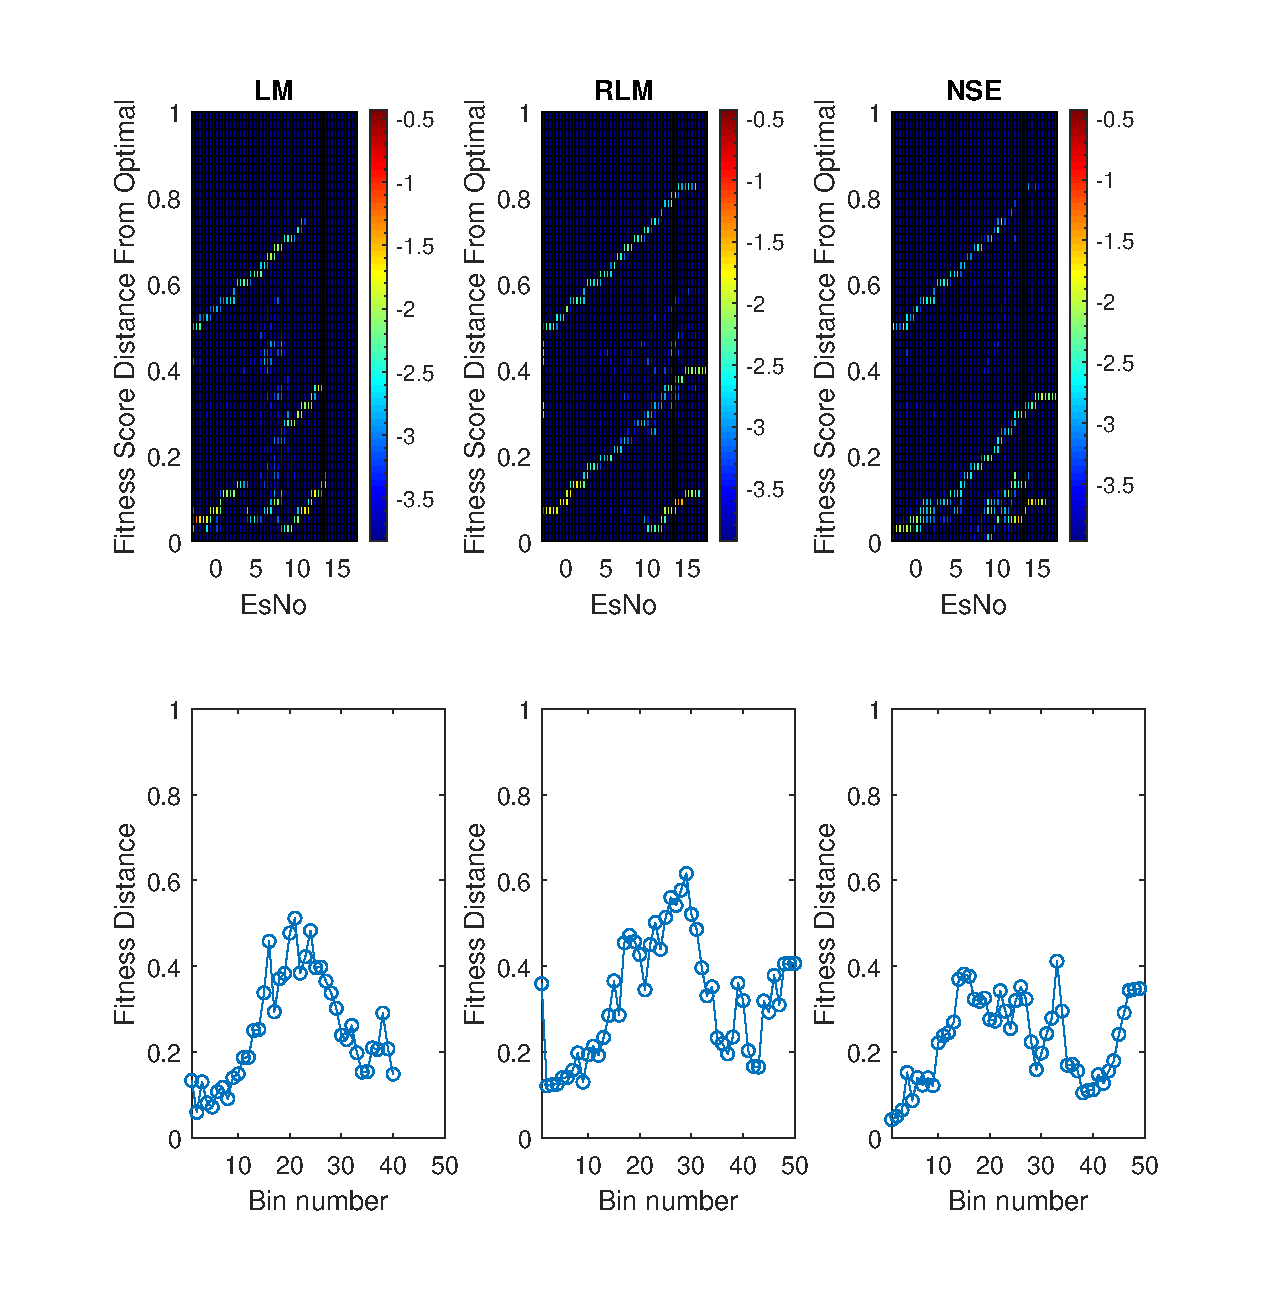
\includegraphics[width=\textwidth]{figures/flight_results/Coop_good_overview.eps}
\caption{Placeholder}
\end{figure}


\begin{itemize}
	\item Time series plot.
	\item histogram
	\item rel histogram
	\item 2d hist, rel, log
	\item binned mean
	\item binned median
	\item sum of binned means and binned medians.
	\item Entire work in appendix.
\end{itemize}